% Created by tikzDevice version 0.12.3 on 2019-09-26 18:24:04
% !TEX encoding = UTF-8 Unicode
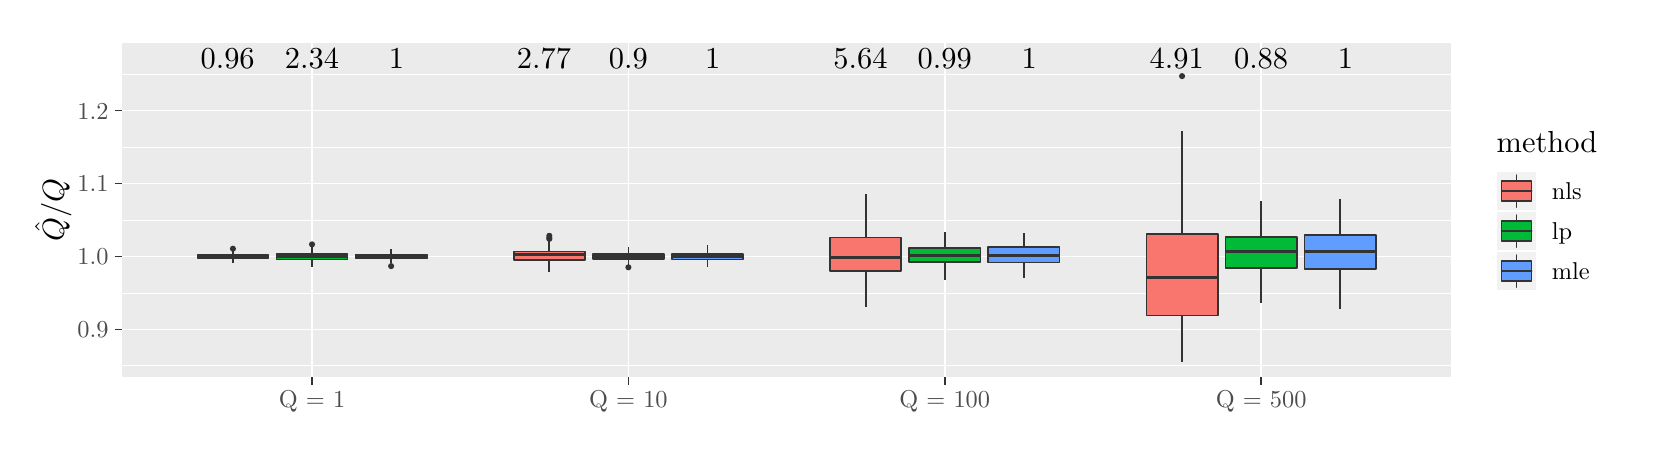
\begin{tikzpicture}[x=1pt,y=1pt]
\definecolor{fillColor}{RGB}{255,255,255}
\path[use as bounding box,fill=fillColor,fill opacity=0.00] (0,0) rectangle (578.16,144.54);
\begin{scope}
\path[clip] (  0.00,  0.00) rectangle (578.16,144.54);
\definecolor{drawColor}{RGB}{255,255,255}
\definecolor{fillColor}{RGB}{255,255,255}

\path[draw=drawColor,line width= 0.6pt,line join=round,line cap=round,fill=fillColor] (  0.00,  0.00) rectangle (578.16,144.54);
\end{scope}
\begin{scope}
\path[clip] ( 34.16, 18.22) rectangle (514.31,139.04);
\definecolor{fillColor}{gray}{0.92}

\path[fill=fillColor] ( 34.16, 18.22) rectangle (514.31,139.04);
\definecolor{drawColor}{RGB}{255,255,255}

\path[draw=drawColor,line width= 0.3pt,line join=round] ( 34.16, 22.32) --
	(514.31, 22.32);

\path[draw=drawColor,line width= 0.3pt,line join=round] ( 34.16, 48.67) --
	(514.31, 48.67);

\path[draw=drawColor,line width= 0.3pt,line join=round] ( 34.16, 75.03) --
	(514.31, 75.03);

\path[draw=drawColor,line width= 0.3pt,line join=round] ( 34.16,101.38) --
	(514.31,101.38);

\path[draw=drawColor,line width= 0.3pt,line join=round] ( 34.16,127.74) --
	(514.31,127.74);

\path[draw=drawColor,line width= 0.6pt,line join=round] ( 34.16, 35.50) --
	(514.31, 35.50);

\path[draw=drawColor,line width= 0.6pt,line join=round] ( 34.16, 61.85) --
	(514.31, 61.85);

\path[draw=drawColor,line width= 0.6pt,line join=round] ( 34.16, 88.21) --
	(514.31, 88.21);

\path[draw=drawColor,line width= 0.6pt,line join=round] ( 34.16,114.56) --
	(514.31,114.56);

\path[draw=drawColor,line width= 0.6pt,line join=round] (102.75, 18.22) --
	(102.75,139.04);

\path[draw=drawColor,line width= 0.6pt,line join=round] (217.07, 18.22) --
	(217.07,139.04);

\path[draw=drawColor,line width= 0.6pt,line join=round] (331.39, 18.22) --
	(331.39,139.04);

\path[draw=drawColor,line width= 0.6pt,line join=round] (445.71, 18.22) --
	(445.71,139.04);
\definecolor{drawColor}{gray}{0.20}
\definecolor{fillColor}{gray}{0.20}

\path[draw=drawColor,line width= 0.4pt,line join=round,line cap=round,fill=fillColor] ( 74.17, 64.67) circle (  0.89);

\path[draw=drawColor,line width= 0.6pt,line join=round] ( 74.17, 62.49) -- ( 74.17, 64.25);

\path[draw=drawColor,line width= 0.6pt,line join=round] ( 74.17, 61.27) -- ( 74.17, 59.57);
\definecolor{fillColor}{RGB}{248,118,109}

\path[draw=drawColor,line width= 0.6pt,line join=round,line cap=round,fill=fillColor] ( 61.31, 62.49) --
	( 61.31, 61.27) --
	( 87.03, 61.27) --
	( 87.03, 62.49) --
	( 61.31, 62.49) --
	cycle;

\path[draw=drawColor,line width= 1.1pt,line join=round] ( 61.31, 61.86) -- ( 87.03, 61.86);
\definecolor{fillColor}{gray}{0.20}

\path[draw=drawColor,line width= 0.4pt,line join=round,line cap=round,fill=fillColor] (102.75, 66.24) circle (  0.89);

\path[draw=drawColor,line width= 0.6pt,line join=round] (102.75, 62.76) -- (102.75, 65.43);

\path[draw=drawColor,line width= 0.6pt,line join=round] (102.75, 60.80) -- (102.75, 58.03);
\definecolor{fillColor}{RGB}{0,186,56}

\path[draw=drawColor,line width= 0.6pt,line join=round,line cap=round,fill=fillColor] ( 89.89, 62.76) --
	( 89.89, 60.80) --
	(115.61, 60.80) --
	(115.61, 62.76) --
	( 89.89, 62.76) --
	cycle;

\path[draw=drawColor,line width= 1.1pt,line join=round] ( 89.89, 61.77) -- (115.61, 61.77);
\definecolor{fillColor}{gray}{0.20}

\path[draw=drawColor,line width= 0.4pt,line join=round,line cap=round,fill=fillColor] (131.33, 58.37) circle (  0.89);

\path[draw=drawColor,line width= 0.6pt,line join=round] (131.33, 62.52) -- (131.33, 64.49);

\path[draw=drawColor,line width= 0.6pt,line join=round] (131.33, 61.13) -- (131.33, 59.47);
\definecolor{fillColor}{RGB}{97,156,255}

\path[draw=drawColor,line width= 0.6pt,line join=round,line cap=round,fill=fillColor] (118.47, 62.52) --
	(118.47, 61.13) --
	(144.19, 61.13) --
	(144.19, 62.52) --
	(118.47, 62.52) --
	cycle;

\path[draw=drawColor,line width= 1.1pt,line join=round] (118.47, 61.85) -- (144.19, 61.85);
\definecolor{fillColor}{gray}{0.20}

\path[draw=drawColor,line width= 0.4pt,line join=round,line cap=round,fill=fillColor] (188.49, 68.60) circle (  0.89);

\path[draw=drawColor,line width= 0.4pt,line join=round,line cap=round,fill=fillColor] (188.49, 68.21) circle (  0.89);

\path[draw=drawColor,line width= 0.4pt,line join=round,line cap=round,fill=fillColor] (188.49, 69.35) circle (  0.89);

\path[draw=drawColor,line width= 0.6pt,line join=round] (188.49, 63.60) -- (188.49, 67.62);

\path[draw=drawColor,line width= 0.6pt,line join=round] (188.49, 60.59) -- (188.49, 56.43);
\definecolor{fillColor}{RGB}{248,118,109}

\path[draw=drawColor,line width= 0.6pt,line join=round,line cap=round,fill=fillColor] (175.63, 63.60) --
	(175.63, 60.59) --
	(201.35, 60.59) --
	(201.35, 63.60) --
	(175.63, 63.60) --
	cycle;

\path[draw=drawColor,line width= 1.1pt,line join=round] (175.63, 62.54) -- (201.35, 62.54);
\definecolor{fillColor}{gray}{0.20}

\path[draw=drawColor,line width= 0.4pt,line join=round,line cap=round,fill=fillColor] (217.07, 57.95) circle (  0.89);

\path[draw=drawColor,line width= 0.6pt,line join=round] (217.07, 62.84) -- (217.07, 65.27);

\path[draw=drawColor,line width= 0.6pt,line join=round] (217.07, 60.91) -- (217.07, 58.72);
\definecolor{fillColor}{RGB}{0,186,56}

\path[draw=drawColor,line width= 0.6pt,line join=round,line cap=round,fill=fillColor] (204.21, 62.84) --
	(204.21, 60.91) --
	(229.93, 60.91) --
	(229.93, 62.84) --
	(204.21, 62.84) --
	cycle;

\path[draw=drawColor,line width= 1.1pt,line join=round] (204.21, 61.97) -- (229.93, 61.97);

\path[draw=drawColor,line width= 0.6pt,line join=round] (245.65, 62.83) -- (245.65, 65.88);

\path[draw=drawColor,line width= 0.6pt,line join=round] (245.65, 60.79) -- (245.65, 58.09);
\definecolor{fillColor}{RGB}{97,156,255}

\path[draw=drawColor,line width= 0.6pt,line join=round,line cap=round,fill=fillColor] (232.79, 62.83) --
	(232.79, 60.79) --
	(258.51, 60.79) --
	(258.51, 62.83) --
	(232.79, 62.83) --
	cycle;

\path[draw=drawColor,line width= 1.1pt,line join=round] (232.79, 61.80) -- (258.51, 61.80);

\path[draw=drawColor,line width= 0.6pt,line join=round] (302.81, 68.71) -- (302.81, 84.36);

\path[draw=drawColor,line width= 0.6pt,line join=round] (302.81, 56.68) -- (302.81, 43.68);
\definecolor{fillColor}{RGB}{248,118,109}

\path[draw=drawColor,line width= 0.6pt,line join=round,line cap=round,fill=fillColor] (289.95, 68.71) --
	(289.95, 56.68) --
	(315.67, 56.68) --
	(315.67, 68.71) --
	(289.95, 68.71) --
	cycle;

\path[draw=drawColor,line width= 1.1pt,line join=round] (289.95, 61.58) -- (315.67, 61.58);

\path[draw=drawColor,line width= 0.6pt,line join=round] (331.39, 64.97) -- (331.39, 70.69);

\path[draw=drawColor,line width= 0.6pt,line join=round] (331.39, 59.76) -- (331.39, 53.40);
\definecolor{fillColor}{RGB}{0,186,56}

\path[draw=drawColor,line width= 0.6pt,line join=round,line cap=round,fill=fillColor] (318.53, 64.97) --
	(318.53, 59.76) --
	(344.25, 59.76) --
	(344.25, 64.97) --
	(318.53, 64.97) --
	cycle;

\path[draw=drawColor,line width= 1.1pt,line join=round] (318.53, 62.19) -- (344.25, 62.19);

\path[draw=drawColor,line width= 0.6pt,line join=round] (359.97, 65.33) -- (359.97, 70.50);

\path[draw=drawColor,line width= 0.6pt,line join=round] (359.97, 59.73) -- (359.97, 54.24);
\definecolor{fillColor}{RGB}{97,156,255}

\path[draw=drawColor,line width= 0.6pt,line join=round,line cap=round,fill=fillColor] (347.11, 65.33) --
	(347.11, 59.73) --
	(372.83, 59.73) --
	(372.83, 65.33) --
	(347.11, 65.33) --
	cycle;

\path[draw=drawColor,line width= 1.1pt,line join=round] (347.11, 62.36) -- (372.83, 62.36);
\definecolor{fillColor}{gray}{0.20}

\path[draw=drawColor,line width= 0.4pt,line join=round,line cap=round,fill=fillColor] (417.13,127.03) circle (  0.89);

\path[draw=drawColor,line width= 0.6pt,line join=round] (417.13, 69.96) -- (417.13,107.22);

\path[draw=drawColor,line width= 0.6pt,line join=round] (417.13, 40.58) -- (417.13, 23.71);
\definecolor{fillColor}{RGB}{248,118,109}

\path[draw=drawColor,line width= 0.6pt,line join=round,line cap=round,fill=fillColor] (404.27, 69.96) --
	(404.27, 40.58) --
	(430.00, 40.58) --
	(430.00, 69.96) --
	(404.27, 69.96) --
	cycle;

\path[draw=drawColor,line width= 1.1pt,line join=round] (404.27, 54.30) -- (430.00, 54.30);

\path[draw=drawColor,line width= 0.6pt,line join=round] (445.71, 68.85) -- (445.71, 81.93);

\path[draw=drawColor,line width= 0.6pt,line join=round] (445.71, 57.65) -- (445.71, 45.17);
\definecolor{fillColor}{RGB}{0,186,56}

\path[draw=drawColor,line width= 0.6pt,line join=round,line cap=round,fill=fillColor] (432.85, 68.85) --
	(432.85, 57.65) --
	(458.58, 57.65) --
	(458.58, 68.85) --
	(432.85, 68.85) --
	cycle;

\path[draw=drawColor,line width= 1.1pt,line join=round] (432.85, 63.74) -- (458.58, 63.74);

\path[draw=drawColor,line width= 0.6pt,line join=round] (474.29, 69.61) -- (474.29, 82.55);

\path[draw=drawColor,line width= 0.6pt,line join=round] (474.29, 57.22) -- (474.29, 42.94);
\definecolor{fillColor}{RGB}{97,156,255}

\path[draw=drawColor,line width= 0.6pt,line join=round,line cap=round,fill=fillColor] (461.43, 69.61) --
	(461.43, 57.22) --
	(487.16, 57.22) --
	(487.16, 69.61) --
	(461.43, 69.61) --
	cycle;

\path[draw=drawColor,line width= 1.1pt,line join=round] (461.43, 63.56) -- (487.16, 63.56);
\definecolor{drawColor}{RGB}{0,0,0}

\node[text=drawColor,anchor=base,inner sep=0pt, outer sep=0pt, scale=  1.10] at (133.23,129.75) {1};

\node[text=drawColor,anchor=base,inner sep=0pt, outer sep=0pt, scale=  1.10] at (102.75,129.75) {2.34};

\node[text=drawColor,anchor=base,inner sep=0pt, outer sep=0pt, scale=  1.10] at ( 72.26,129.75) {0.96};

\node[text=drawColor,anchor=base,inner sep=0pt, outer sep=0pt, scale=  1.10] at (247.56,129.75) {1};

\node[text=drawColor,anchor=base,inner sep=0pt, outer sep=0pt, scale=  1.10] at (217.07,129.75) {0.9};

\node[text=drawColor,anchor=base,inner sep=0pt, outer sep=0pt, scale=  1.10] at (186.59,129.75) {2.77};

\node[text=drawColor,anchor=base,inner sep=0pt, outer sep=0pt, scale=  1.10] at (361.88,129.75) {1};

\node[text=drawColor,anchor=base,inner sep=0pt, outer sep=0pt, scale=  1.10] at (331.39,129.75) {0.99};

\node[text=drawColor,anchor=base,inner sep=0pt, outer sep=0pt, scale=  1.10] at (300.91,129.75) {5.64};

\node[text=drawColor,anchor=base,inner sep=0pt, outer sep=0pt, scale=  1.10] at (476.20,129.75) {1};

\node[text=drawColor,anchor=base,inner sep=0pt, outer sep=0pt, scale=  1.10] at (445.71,129.75) {0.88};

\node[text=drawColor,anchor=base,inner sep=0pt, outer sep=0pt, scale=  1.10] at (415.23,129.75) {4.91};
\end{scope}
\begin{scope}
\path[clip] (  0.00,  0.00) rectangle (578.16,144.54);
\definecolor{drawColor}{gray}{0.30}

\node[text=drawColor,anchor=base east,inner sep=0pt, outer sep=0pt, scale=  0.88] at ( 29.21, 32.47) {0.9};

\node[text=drawColor,anchor=base east,inner sep=0pt, outer sep=0pt, scale=  0.88] at ( 29.21, 58.82) {1.0};

\node[text=drawColor,anchor=base east,inner sep=0pt, outer sep=0pt, scale=  0.88] at ( 29.21, 85.18) {1.1};

\node[text=drawColor,anchor=base east,inner sep=0pt, outer sep=0pt, scale=  0.88] at ( 29.21,111.53) {1.2};
\end{scope}
\begin{scope}
\path[clip] (  0.00,  0.00) rectangle (578.16,144.54);
\definecolor{drawColor}{gray}{0.20}

\path[draw=drawColor,line width= 0.6pt,line join=round] ( 31.41, 35.50) --
	( 34.16, 35.50);

\path[draw=drawColor,line width= 0.6pt,line join=round] ( 31.41, 61.85) --
	( 34.16, 61.85);

\path[draw=drawColor,line width= 0.6pt,line join=round] ( 31.41, 88.21) --
	( 34.16, 88.21);

\path[draw=drawColor,line width= 0.6pt,line join=round] ( 31.41,114.56) --
	( 34.16,114.56);
\end{scope}
\begin{scope}
\path[clip] (  0.00,  0.00) rectangle (578.16,144.54);
\definecolor{drawColor}{gray}{0.20}

\path[draw=drawColor,line width= 0.6pt,line join=round] (102.75, 15.47) --
	(102.75, 18.22);

\path[draw=drawColor,line width= 0.6pt,line join=round] (217.07, 15.47) --
	(217.07, 18.22);

\path[draw=drawColor,line width= 0.6pt,line join=round] (331.39, 15.47) --
	(331.39, 18.22);

\path[draw=drawColor,line width= 0.6pt,line join=round] (445.71, 15.47) --
	(445.71, 18.22);
\end{scope}
\begin{scope}
\path[clip] (  0.00,  0.00) rectangle (578.16,144.54);
\definecolor{drawColor}{gray}{0.30}

\node[text=drawColor,anchor=base,inner sep=0pt, outer sep=0pt, scale=  0.88] at (102.75,  7.21) {Q = 1};

\node[text=drawColor,anchor=base,inner sep=0pt, outer sep=0pt, scale=  0.88] at (217.07,  7.21) {Q = 10};

\node[text=drawColor,anchor=base,inner sep=0pt, outer sep=0pt, scale=  0.88] at (331.39,  7.21) {Q = 100};

\node[text=drawColor,anchor=base,inner sep=0pt, outer sep=0pt, scale=  0.88] at (445.71,  7.21) {Q = 500};
\end{scope}
\begin{scope}
\path[clip] (  0.00,  0.00) rectangle (578.16,144.54);
\definecolor{drawColor}{RGB}{0,0,0}

\node[text=drawColor,rotate= 90.00,anchor=base,inner sep=0pt, outer sep=0pt, scale=  1.10] at ( 13.08, 78.63) {$\hat{Q}/Q$};
\end{scope}
\begin{scope}
\path[clip] (  0.00,  0.00) rectangle (578.16,144.54);
\definecolor{fillColor}{RGB}{255,255,255}

\path[fill=fillColor] (525.31, 43.84) rectangle (572.66,113.42);
\end{scope}
\begin{scope}
\path[clip] (  0.00,  0.00) rectangle (578.16,144.54);
\definecolor{drawColor}{RGB}{0,0,0}

\node[text=drawColor,anchor=base west,inner sep=0pt, outer sep=0pt, scale=  1.10] at (530.81, 99.27) {method};
\end{scope}
\begin{scope}
\path[clip] (  0.00,  0.00) rectangle (578.16,144.54);
\definecolor{drawColor}{RGB}{255,255,255}
\definecolor{fillColor}{gray}{0.95}

\path[draw=drawColor,line width= 0.6pt,line join=round,line cap=round,fill=fillColor] (530.81, 78.25) rectangle (545.26, 92.70);
\end{scope}
\begin{scope}
\path[clip] (  0.00,  0.00) rectangle (578.16,144.54);
\definecolor{drawColor}{gray}{0.20}

\path[draw=drawColor,line width= 0.6pt,line join=round,line cap=round] (538.03, 79.70) --
	(538.03, 81.86);

\path[draw=drawColor,line width= 0.6pt,line join=round,line cap=round] (538.03, 89.09) --
	(538.03, 91.26);
\definecolor{fillColor}{RGB}{248,118,109}

\path[draw=drawColor,line width= 0.6pt,line join=round,line cap=round,fill=fillColor] (532.61, 81.86) rectangle (543.45, 89.09);

\path[draw=drawColor,line width= 0.6pt,line join=round,line cap=round] (532.61, 85.48) --
	(543.45, 85.48);
\end{scope}
\begin{scope}
\path[clip] (  0.00,  0.00) rectangle (578.16,144.54);
\definecolor{drawColor}{RGB}{255,255,255}
\definecolor{fillColor}{gray}{0.95}

\path[draw=drawColor,line width= 0.6pt,line join=round,line cap=round,fill=fillColor] (530.81, 63.80) rectangle (545.26, 78.25);
\end{scope}
\begin{scope}
\path[clip] (  0.00,  0.00) rectangle (578.16,144.54);
\definecolor{drawColor}{gray}{0.20}

\path[draw=drawColor,line width= 0.6pt,line join=round,line cap=round] (538.03, 65.24) --
	(538.03, 67.41);

\path[draw=drawColor,line width= 0.6pt,line join=round,line cap=round] (538.03, 74.64) --
	(538.03, 76.81);
\definecolor{fillColor}{RGB}{0,186,56}

\path[draw=drawColor,line width= 0.6pt,line join=round,line cap=round,fill=fillColor] (532.61, 67.41) rectangle (543.45, 74.64);

\path[draw=drawColor,line width= 0.6pt,line join=round,line cap=round] (532.61, 71.02) --
	(543.45, 71.02);
\end{scope}
\begin{scope}
\path[clip] (  0.00,  0.00) rectangle (578.16,144.54);
\definecolor{drawColor}{RGB}{255,255,255}
\definecolor{fillColor}{gray}{0.95}

\path[draw=drawColor,line width= 0.6pt,line join=round,line cap=round,fill=fillColor] (530.81, 49.34) rectangle (545.26, 63.80);
\end{scope}
\begin{scope}
\path[clip] (  0.00,  0.00) rectangle (578.16,144.54);
\definecolor{drawColor}{gray}{0.20}

\path[draw=drawColor,line width= 0.6pt,line join=round,line cap=round] (538.03, 50.79) --
	(538.03, 52.96);

\path[draw=drawColor,line width= 0.6pt,line join=round,line cap=round] (538.03, 60.18) --
	(538.03, 62.35);
\definecolor{fillColor}{RGB}{97,156,255}

\path[draw=drawColor,line width= 0.6pt,line join=round,line cap=round,fill=fillColor] (532.61, 52.96) rectangle (543.45, 60.18);

\path[draw=drawColor,line width= 0.6pt,line join=round,line cap=round] (532.61, 56.57) --
	(543.45, 56.57);
\end{scope}
\begin{scope}
\path[clip] (  0.00,  0.00) rectangle (578.16,144.54);
\definecolor{drawColor}{RGB}{0,0,0}

\node[text=drawColor,anchor=base west,inner sep=0pt, outer sep=0pt, scale=  0.88] at (550.76, 82.45) {nls};
\end{scope}
\begin{scope}
\path[clip] (  0.00,  0.00) rectangle (578.16,144.54);
\definecolor{drawColor}{RGB}{0,0,0}

\node[text=drawColor,anchor=base west,inner sep=0pt, outer sep=0pt, scale=  0.88] at (550.76, 67.99) {lp};
\end{scope}
\begin{scope}
\path[clip] (  0.00,  0.00) rectangle (578.16,144.54);
\definecolor{drawColor}{RGB}{0,0,0}

\node[text=drawColor,anchor=base west,inner sep=0pt, outer sep=0pt, scale=  0.88] at (550.76, 53.54) {mle};
\end{scope}
\end{tikzpicture}
